% Ubah kalimat sesuai dengan judul dari bab ini
\chapter{PROFIL PERUSAHAAN}

% Ubah konten-konten berikut sesuai dengan yang ingin diisi pada bab ini

\section{Profil Laboratorium MCI}

\begin{figure}[H]
	\centering
	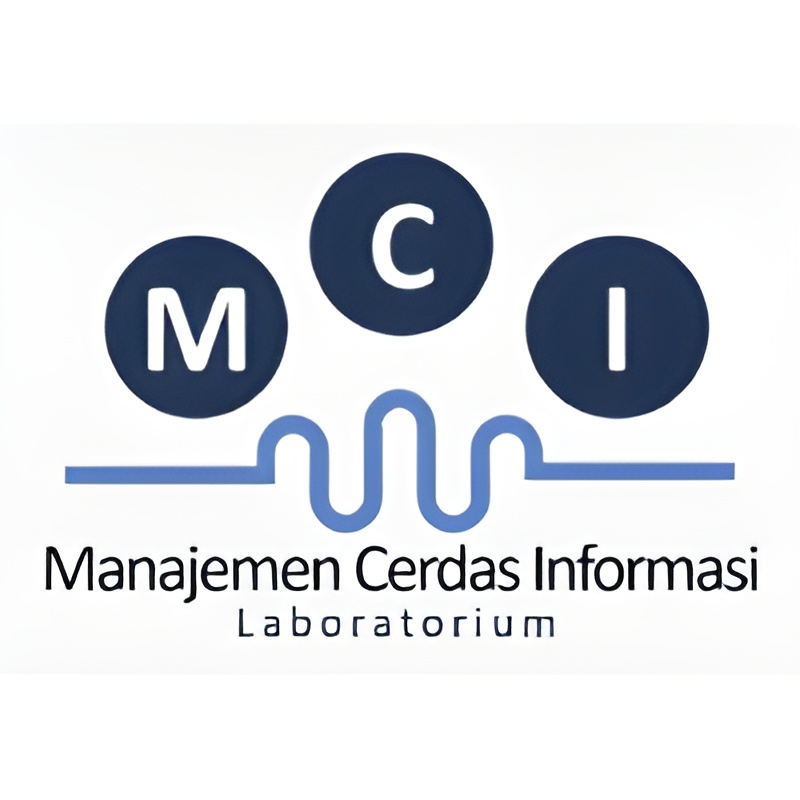
\includegraphics[width=0.55\linewidth]{gambar/logo-mci.png}
	\caption{Logo Laboratorium MCI}
	\label{fig:logo-mci}
\end{figure}

Laboratorium Manajemen Cerdas Informasi (MCI) menawarkan bidang keahlian yang ditekankan pada kemampuan lulusan dalam menganalisis, mensintesa dan mengevaluasi proses bisnis dan sistem informasi pada sistem Enterprise, mengimplementasikan rekayasa pengetahuan ke dalam suatu aplikasi, melakukan investigasi, pengujian, evaluasi kematangan dan kepatutan terhadap prosedur standar dan tata kelola teknologi informasi, melakukan tata kelola proyek dan sumber daya manusia dan merancang dan mengimplementasikan solusi basis data terdistribusi dan teknologi \textit{Big Data}. Mata kuliah bidang keahlian dibawah naungan MCI antara lain, Sistem Enterprise, Rekayasa Pengetahuan, Sistem Informasi Geografis, Audit Sistem, Tata Kelola Teknologi Informasi, Basis Data Terdistribusi, Big Data, Topik Khusus Manajemen Informasi.

%\section{Visi dan Misi}

\section{Lokasi Laboratorium MCI}

Laboratorium MCI berlokasi di Jalan Teknik Kimia - Gedung Departemen Teknik Informatika,  Kampus Institut Teknologi Sepuluh Nopember Jalan Raya ITS, Sukolilo, Surabaya 60111, Indonesia.

\section{Struktur Organisasi Laboratorium MCI}

Laboratorium MCI dipimpin oleh ketua laboratorium dan terdiri dosen anggota. Gambar \ref{fig:struktur-organisasi} menunjukkan struktur organisasi laboratorium MCI.

\begin{figure}[H]
	\centering
	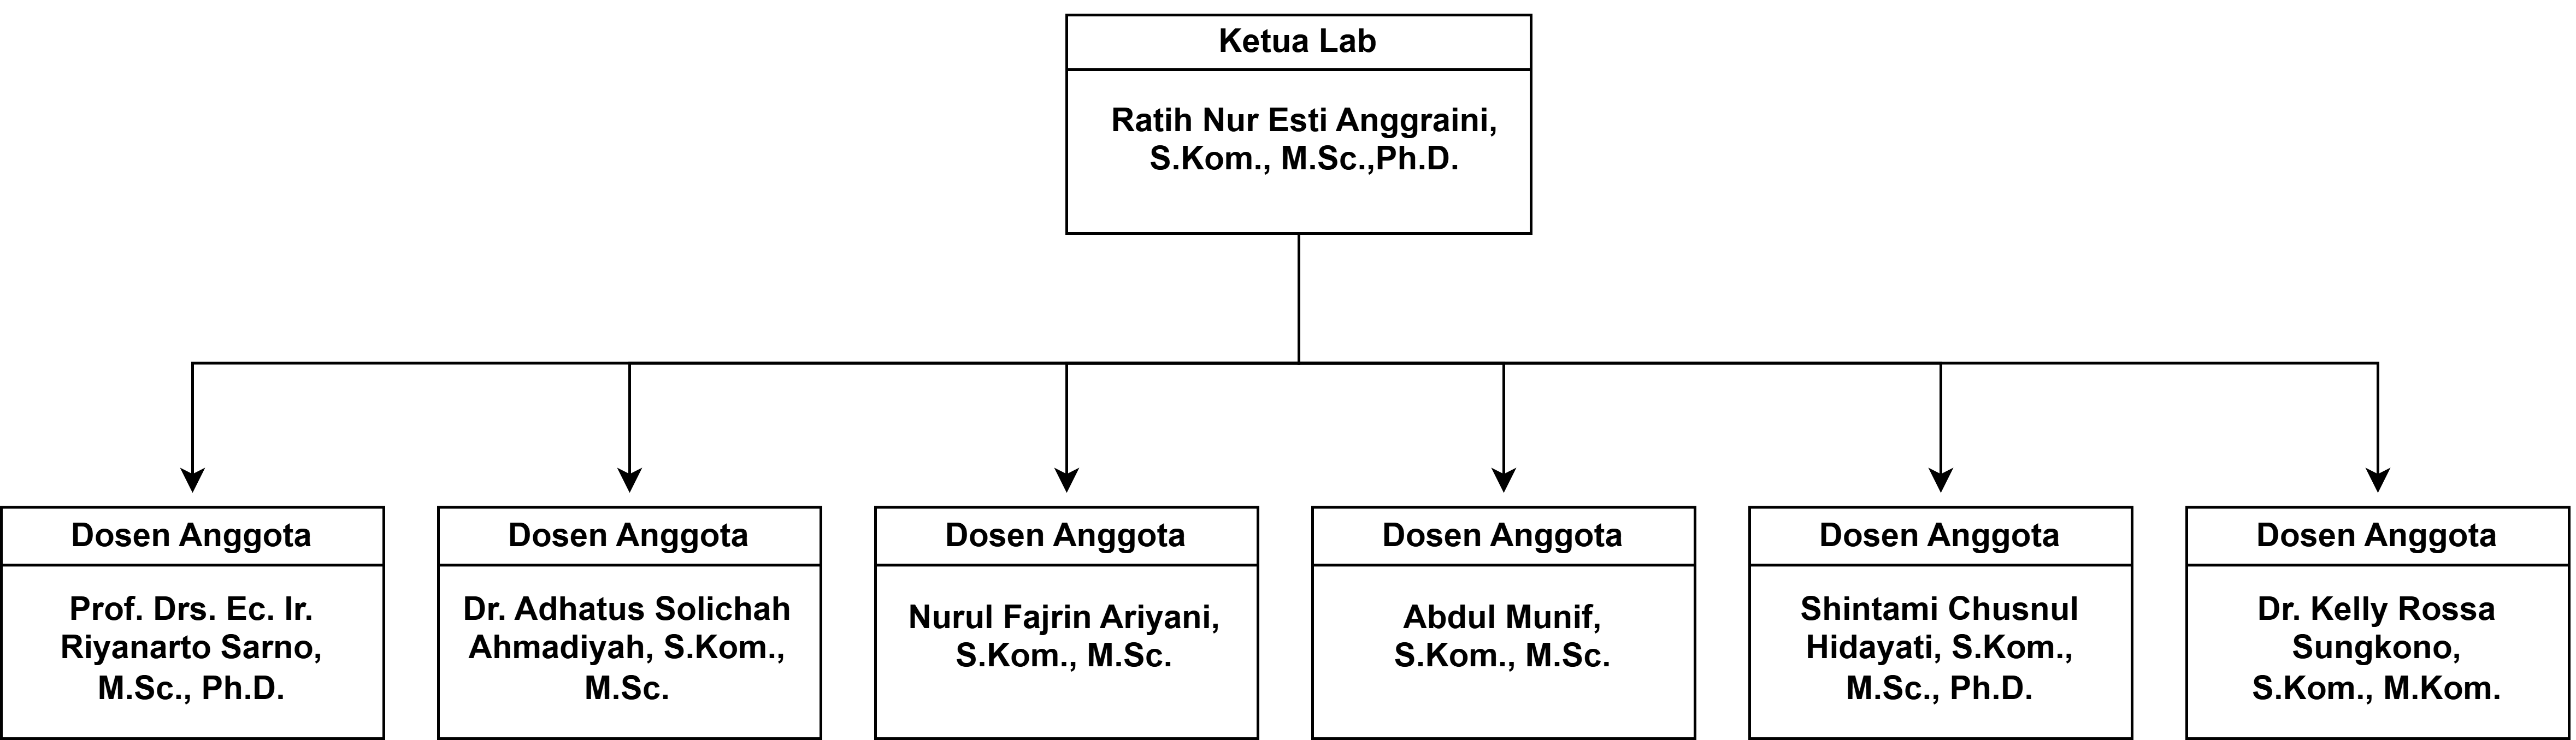
\includegraphics[width=\linewidth]{gambar/struktur-organisasi-mci.png}
	\caption{Struktur Organisasi Laboratorium MCI}
	\label{fig:struktur-organisasi}
\end{figure} 